%!TEX root = paper.tex

Rather than looking at an explicit representation of lines in the plane, we can gain much more insight from looking at a parametric representation. To simplify our analysis, we will choose our time parameter such that v collisions occur every $\Delta t = 1$ and h collisions occur every $\Delta t = m$. The equation for a line $y(x) = m \, x + b$ is equivalent to the following parametric system

\begin{align}\label{eq:parametric-line}
	x(t)& = \frac{1}{m} \, t + x_0\\
	y(t)& = t
\end{align}

Now our v and h collisions in the 2-dimensional plane can be projected onto the 1-dimensional $t$ axis.

\begin{figure}[H]
  \begin{center}
    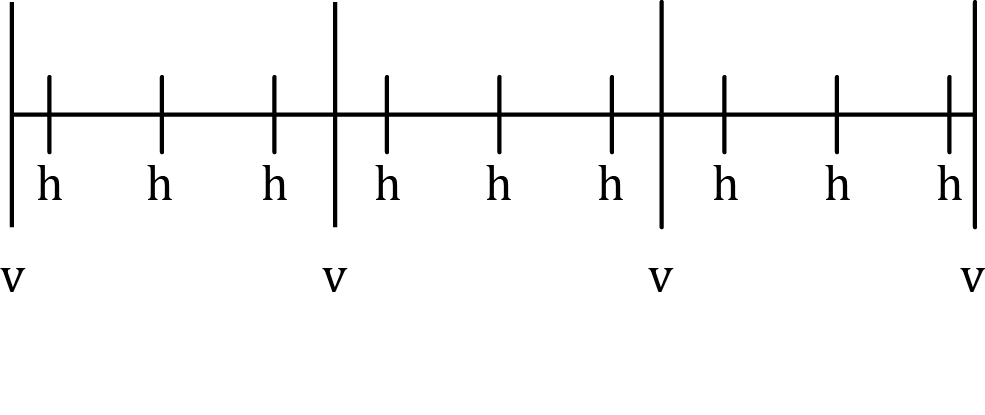
\includegraphics[keepaspectratio, width=4in]{1d_mapping_2.png}
  \end{center}
  \vspace{-.2in} % corrects bad spacing
  \caption{\label{fig:1d-projection} Projecting onto the parametric representation.}
\end{figure}

\begin{lemma}\label{lemma:h-extension}
	A finite sequence $\alpha$ is a valid collision sequence iff there exists at least one valid collision sequence containing $\alpha$ that starts and ends with an h.
\end{lemma}

\begin{proof}
	TODO
\end{proof}

Because of Lemma \ref{lemma:h-extension}, without loss of generality we can confine ourselves to only look at collision sequences that start and end with an h.

\begin{definition}
	Given a collision sequence $\alpha$, define a sequence $\beta$ where each element $\beta^{(0)}_i$ is the number of v collisions between the i\textsuperscript{th} and (i+1)\textsuperscript{th} h in $\alpha$.
\end{definition}

The $\beta^{(0)}$ sequence is much simpler to think of geometrically: $\beta^{(0)}_i$ represents the number of v collision tick marks in between each h collision tick mark which is shown in Figure \ref{fig:beta-sequence}.

\begin{figure}[H]
  \begin{center}
    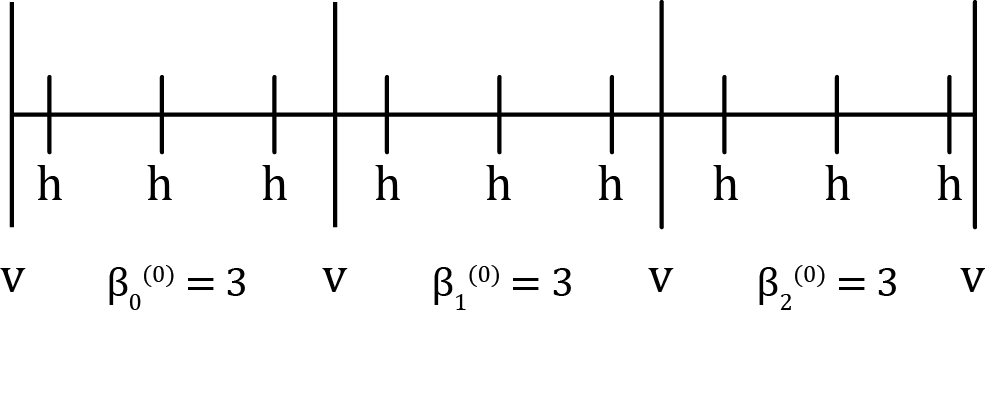
\includegraphics[keepaspectratio, width=4in]{1d_mapping_3.png}
  \end{center}
  \vspace{-.2in} % corrects bad spacing
  \caption{\label{fig:beta-sequence} The $\beta^{(i)}$ sequence.}
\end{figure}

\begin{theorem}\label{thm:beta_exremum}
	For every valid collision sequence, the following must be true
	
	\begin{equation}
		\beta^{(0)}_{max} - \beta^{(0)}_{min} \le 1
	\end{equation}
\end{theorem}

\begin{proof}

From Equation \ref{eq:parametric-line}, v collisions occur every $\Delta t = 1$ and h collisions occur every $\Delta t = m$. Thus, the following must be true

\begin{equation}
	\beta^{(0)}_i \in \paren{\floor{m}, \ceil{m}}
\end{equation}

For an $m$ to exist that satisfies the above constraints, all numbers in the $\beta$ sequence can only differ by 1.

\end{proof}

\begin{definition}
	Given a valid collision sequence, define the sequence $\beta^{(j)}$ where each element $\beta^{(j)}_i$ is 1 more than the number of occurrences of $\beta^{(j-1)}_{max}$ between the i\textsuperscript{th} and (i+1)\textsuperscript{th} occurrence of $\beta^{(j-1)}_{min}$ in the $\beta^{(j-1)}$ sequence.

	If, for some $j_f$, the length of $\beta^{(j_f-1)}$ is 1, then $\beta^{(j_f-1)}$ is the terminating \"meta\" sequence, and all subsequent $\beta^{(j)}$ for $j \ge j_f$ are undefined.
\end{definition}

\begin{definition}
	Define the sequence $a$ in the following manner

	\begin{equation}
		a_j \coloneqq \begin{cases}
			m \qquad &\text{for} \quad j = 0\\
			1 \qquad &\text{for} \quad j = 1\\
			\beta^{(j-2)}_{max} a_{j-1} - a_{j-2} \qquad &\text{for} \quad 2 \le j < j_f
		\end{cases}
	\end{equation}

\end{definition}

From now on we will only consider collision sequences, where each $\beta^{(j)}$ either starts and ends with $\beta^{(j)}_{min}$ or has length 1.

\begin{theorem}\label{thm:beta_i}
	A collision sequence is valid iff the following is true for all $j$

	\begin{equation}
		\beta^{(j)}_i \in \cbracket{\floor{\frac{a_{j-2}}{a_{j-1}}}, \ceil{\frac{a_{j-2}}{a_{j-1}}}}
	\end{equation}
\end{theorem}

\begin{proof}
	If we pick a $\beta^{(j)}_i$ and plot it in the following manner, we notice that  

	Define
	\begin{align}
		\gamma& = \ceil{\frac{a_{j-1}}{a_{j-2}}}\\
		& \ge \frac{a_{j-1}}{a_{j-2}}
	\end{align}


	and
	\begin{align}\label{delta_beta}
			\delta^{(j)}_i \coloneqq \begin{cases}
				x_0 \qquad &\text{for} \quad i = 0\\
				i (\gamma *  - a_{i-2}) + x_0 \qquad &\text{for} i \ge 1
			\end{cases}
	\end{align}

	We can notice that

	\begin{align}\label{eq:beta_i}
		\beta^{(j)}_i = \floor{\delta^{(j)}_i} + \beta^{(j)}_{max} - \floor{\delta^{(j)}_{i+1}}
	\end{align}
\end{proof}

We can immediately notice that the $\delta^{(0)}$ sequence has the following features:

\begin{enumerate}
	\item The $\delta^{(0)}$ sequence is increasing, because $\beta^{(0)}_{max} \ge m$
	\item Combining Theorem \ref{thm:beta_exremum} and Equation \ref{eq:beta_i}, we get the following:

		\begin{align}
			\floor{\delta^{(0)}_{i+1}} - \floor{\delta^{(0)}_{i+1}}& = \beta^{(0)}_{max} - \beta^{(0)}_{min}\\
			& \le 1
		\end{align}
\end{enumerate}

Thus, if we plot the values of the $\delta^{(0)}$ sequence on a line, we notice something interesting: the plot looks very similar to our original plot of the collision sequence parameterized by $t$.

We can continue in this fashion forming more \"meta\" sequences.



\begin{theorem}
	For every valid collision sequence, $a \to 0$
\end{theorem}

\begin{proof}

\end{proof}
